\def\year{2015}
%File: formatting-instruction.tex
\documentclass[letterpaper]{article}
\usepackage{aaai}
\usepackage{times}
\usepackage{helvet}
\usepackage{courier}
%%
\usepackage{graphicx}
\usepackage{url}
\usepackage{amsfonts}
\usepackage{moreverb}
%%
\usepackage{bm}
\usepackage{paralist}
%\usepackage{minted}
%%
% so we don't need to specify figures subdirectory in figure code
\graphicspath{{./figures/}}
\usepackage{subfig}
%needed to change table colors
\usepackage[table]{xcolor}
\renewcommand{\arraystretch}{1.2} % General space between rows (1 standard)

%%
\frenchspacing
\setlength{\pdfpagewidth}{8.5in}
\setlength{\pdfpageheight}{11in}
\pdfinfo{
/Title (Insert Your Title Here)
/Author (Put All Your Authors Here, Separated by Commas)}
\setcounter{secnumdepth}{0}  
 \begin{document}
% The file aaai.sty is the style file for AAAI Press 
% proceedings, working notes, and technical reports.
%
\title{Activity Monitoring and Prediction for Humans and NAO Humanoid Robots using 
Wearable Sensors}
% \author{Author names \\ %Saminda Abeyruwan \and Faisal Sikder \and Dilip Sarkar\\
% University of Miami \\
% Department of Computer Science\\
% 1365 Memorial Drive, Coral Gables, FL, 33146, USA\\
% %{\ttfamily \{saminda|f.sikder|sarkar\}@cs.miami.edu}
% }
\maketitle
\begin{abstract}
\begin{quote}
Monitoring and learning from activities such as jogging, running, falling so forth for humans and 
humanoid biped robots provide predictions to improve the activities as well as to prevent 
accidental or unforeseen situations. The predictions must be delivered within the time scales of 
the activities for gain maximum performance. In order to learn from activities and to provide 
predictions, the two demographic groups are impel to ware external devices with sensors. This 
paper provides: \begin{inparaenum}[1)] \item a generalize method to learn and predict activities 
of the groups; and \item a modular software framework to realize learning/predictions 
efficiently on embedded devices. \end{inparaenum} We have use on/off-line reactive and deliberative 
methods to learn from activities and to provide predictions. Our software development platform has 
been tested on MSP-EXP430G2, Tiva C Series EK-TM4C123GXL, and Tiva C Series TM4C129 Connected 
LaunchPads. It is lightweight, flexible, and consumes minimum memory and computational 
resources to develop applications and rational agents on microcontrollers that sense and actuate 
using add-on boards. We have used our framework to learn from activities and to deliver predictions 
on able-bodied humans and on NAO biped humanoid robots. We empirically evaluate the outcomes and 
show the success of the methods on different activity settings. 
\end{quote}
\end{abstract}

\section{Introduction}
\label{sec:Intro}
The humans as well as the biped humanoid robots complete apparently simple activities that requires 
complex computational tasks. These activities include jogging, running so forth. While performing 
these safe activities, accidents such as falls may occur causing damage to human body or to 
structural components of a humanoid robot \cite{li2009accurate}. There has been an 
increasing demand in domains such as rescue to use autonomous or teleoperated humanoid robots to 
complete high-risk tasks otherwise would have been lethal to a human subject. Therefore, we 
envision environments where humans and humanoid robots collaboratively work to complete 
tasks. 

Since both humans and biped humanoid robots have similar movements and are susceptible to 
similar accidents, we believe that the same set of learning algorithms are suitable for both 
groups. In this paper,  to validate our believes, we develop a generalize approach for learning 
and predictions for activities of both groups.  We have attached wearable sensing devices for 
collecting motion data and have used software tools to interpret the sensor data for distinguishing 
between normal and abnormal activities. The sensing devices are assembled using off-the-shelf 
hardware component boards and the generalize software tools are developed by ourselves to 
collect data for learning and to identify activities. The software tools provide a modular 
functionalities to use for collecting  data from any sensing devices, and to learn and predict 
on/off-line. While attempts for identifying human motions have already been investigated, to the 
best of our knowledge, we are the first to investigate the prospect of using external embedded 
devices to identify activities on a NAO. Before we report our contribution, we provide a brief 
review of work related to identification of human activity.  


\begin{figure*}[!t]
\centering
\subfloat[]{\label{fig:fa}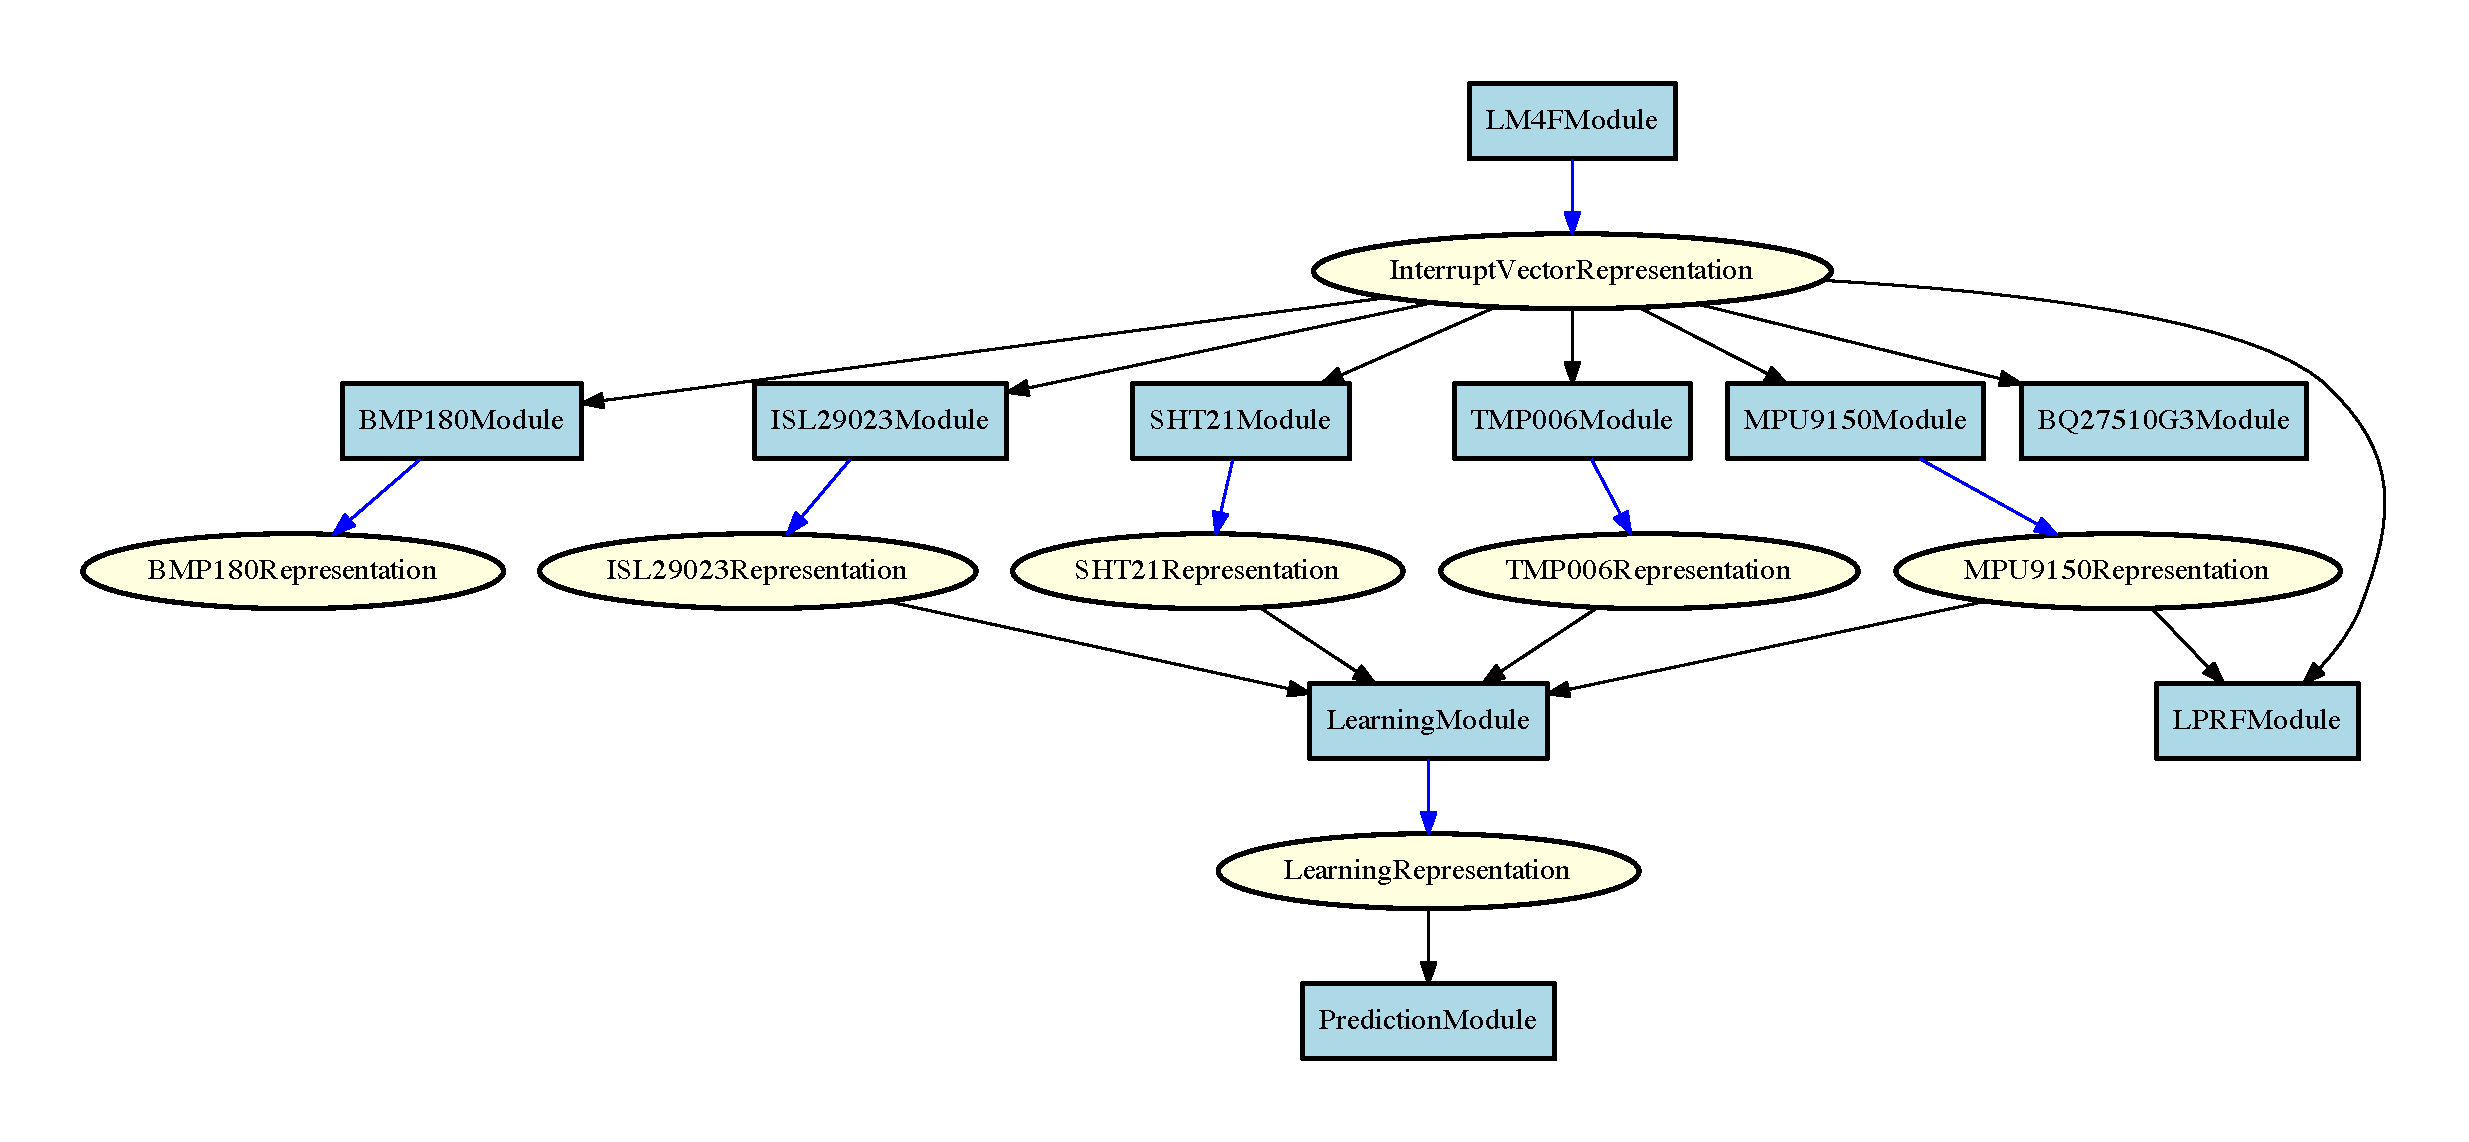
\includegraphics[width=0.6\textwidth]{figures/graph_structure_def-crop2}}
\subfloat[]{\label{fig:fb}\includegraphics[width=0.21\textwidth]{figures/human_figure}}
\subfloat[]{\label{fig:fc}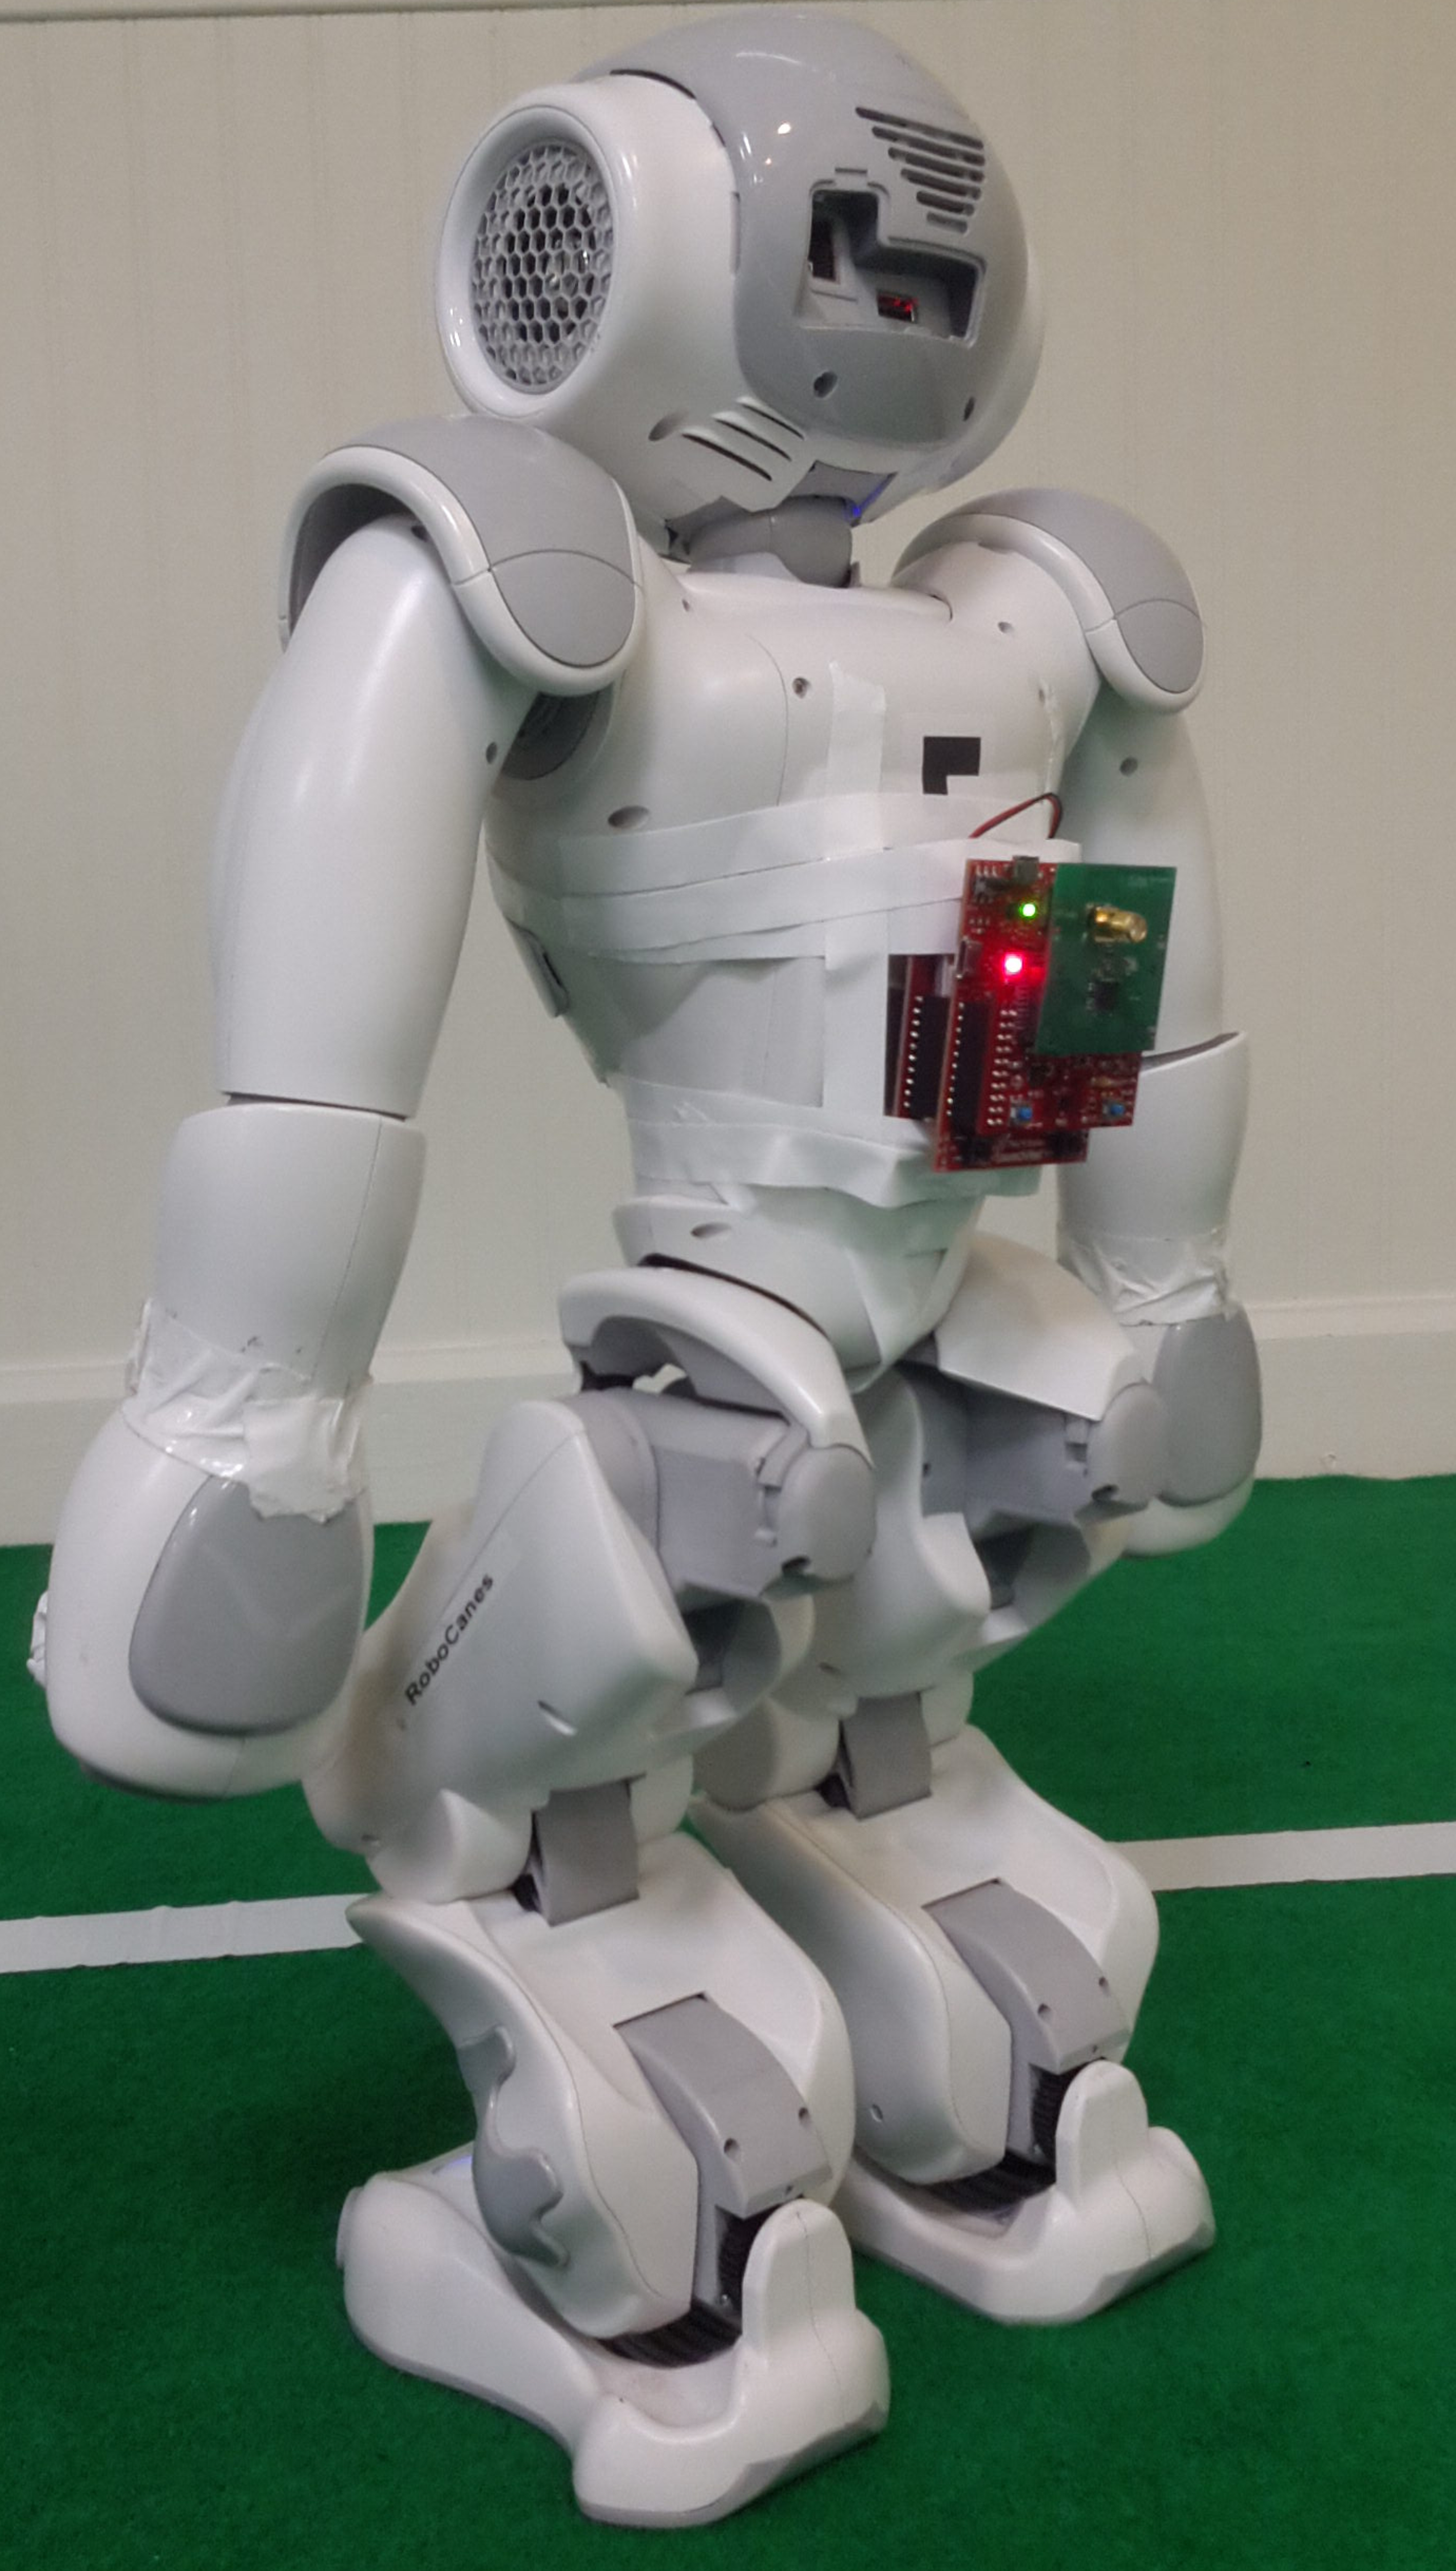
\includegraphics[width=0.185\textwidth]{figures/robot_figure}} 
\caption{(a) The modules and representations used in the experiments;  (b) the wireless transmitter 
was attached to a Sensor Hub BoosterPack on a Tiva C LaunchPad microcontroller that was connected to 
a Fuel Tank BoosterPack, which was then attached to the back of a human subject; and (c) the same 
device configuration was used on the back of a NAO humanoid robot.}
 \label{fig:framework}
\end{figure*}


\subsection{Related Work}

Before we report our contribution, we provide a brief review of work related to identification of 
human activity. 
The existing activity detection methods focus on special cases of fall detection in humans and 
humanoid robots. These methods are primarily used in isolation.  
In SAFE (SmArt Fall dEtection) {~\cite{ojetola2011fall}} researchers used accelerometers and 
gyroscopes 
to detect fall incidence among the elderly people, they have used C4.5 decision tree to learn and 
classify fall and ADLs (activities of daily living). They claimed to identify four different types 
of falls with a precision of 81\% accuracy and recall of 92\% accuracy.
Javier Moya et. al.{~\cite{moya2014fall}} proposed a fall detection, avoidance and damage reduction 
mechanism for biped humanoid robots. They tried to simulate the real world environment where 
humanoid robots have to walk over irregular surface, running or playing sports, collusion with 
other 
robots and according to their article the proposed framework can detect instability and do fall 
avoidance or at least low-damage falling mechanism is invoked. 
%% faisal end

There has been an increasing interest in detecting human motions using embedded devices. Woon-Sung
et. al. \cite{baek2013real} proposed  a fall  detection  system  using necklace-shaped tri-axial
accelerometer  and  gyroscope  sensors  to  classify  the  behavior  and  posture  of  the detection
 subject. They claim that their  approach  can  successfully  distinguish between  ADL and  fall, 
with  sensitivities  greater  than  80 \%  and specificities  of  100\%. Ying-Wen et. al.
\cite{bai2013recognition} proposed an activity monitoring system based on smart phone sensor
reading and they claim that they can identify human activity with high degree of accuracy. Leno et.
al. \cite{leone2013supervised} prosed a system to detect event that cause trauma, and disabilities
using a tri-axial MEMS wearable wireless accelerometer. They have used support vector machine for
robust classification of different events. There has been similar efforts to detect human motions
using motion tracking, e.g., \cite{dumitrache2013fall,kumarwearable,liang2012pre}. The 
microcontrollers and embedded devices provide a flexible platform to build may 
real world applications. 

We have used Texas Instruments (TIs)\footnote{\url{https://www.ti.com/}} 
 microcontrollers and boosterpacks for our 
experiments, but, one can use microcontrollers and sensor boards from other sources.  


%  The microcontrollers and embedded devices provide a flexible platform to build may 
% real world applications. In order to build these applications, a practitioner would require  
% flexible and reliable software solutions. A practitioner also may require to use more than one 
% functionality provided by the devices to build applications. Existing software solutions provide 
% facilities to build applications to a certain degree, but, they lack methods or systems to 
% integrate 
% multiple devices simultaneously without much user burden. We have developed  a state-of-the-art 
% open 
% source software solution to build heterogeneous applications on many devices, which can be 
% programmed on multiple operating systems. 

\subsection{Our Approach and Contributions}

TI microcontrollers  boards such 
as MSP430{\texttrademark}LaunchPad, Tiva{\texttrademark} C Series TM4C123G
LaunchPad, Tiva C Series 
TM4C129 Connected LaunchPad, and add-on booster packs such as Sensor Hub BoosterPack and CC2533 
wireless transmitter and 
receiver  provide flexible platform for developing solutions for a wide rage of low power 
and portable applications. For our experiments, we have assembled a device with Tiva C Series 
TM4C123G microcontroller board, and three boosterpacks. The boosterpacks are for sensing 9-axis 
motion, battery power, and wireless networking. We have used two of the assembled devices to create 
a wireless sensor network (WSN) to collect motion data from  humans and NAO humanoid robots.   

We have developed a set of software tools to create a framework that allow us to: 
\begin{inparaenum}[1)] \item setup the WSN; \item collect data; \item learning; and \item 
prediction. \end{inparaenum} This framework is general enough for other practitioners to use the
available functionalities for creating WSNs, collecting data, learning, and prediction.



%FIXMe latter 
We have used our framework to experiment on the problem of activity detection using InvenSense 
MPU-9150: 9-axis MEMS motion tracking sensor. We have conducted our experiments on able-bodied 
humans and on NAO humanoid robots to detect activities such as standing, walking, and abruptly 
falling back and front. We have used the same device configuration as show in Figures \ref{fig:fb}, 
and \ref{fig:fc}. The wireless transmitter was attached to a Sensor Hub BoosterPack on a Tiva C 
LaunchPad microcontroller that was connected to a Fuel Tank BoosterPack, which was then attached to 
the back of a human subject or a NAO humanoid robot. We have used reactive (e.g., threshold based) 
and deliberative (e.g., machine learning) methods to detect and predict activities. We have 
provided  evaluations and empirical results to  justify the success of our methods. 


\section{Framework}

The framework provides functionalities to 
build  rational agents that perceive its environment though sensors and act upon it though 
actuators. The execution path between sensors to actuators may contain complex behaviors and 
modeling decisions that needs to be handled carefully. Hence, the framework takes these 
consideration into account and provides a topologically sorted graph based on the decision points 
provided by practitioners. Our framework consists for four parts: \begin{inparaenum}[(1)]\item 
processes microcontrollers; \item processes offline processing; \item access functionalities for  
robots; and \item real-time visualizations\end{inparaenum}. The 
framework is lightweight, flexible, and consumes minimum memory and computational resources as 
possible. We have tested our framework on multiple microcontrollers and on boosterpacks as stated 
above. We have written and distributed  software solutions to access devices on the boosterpacks 
such 
as \begin{inparaenum}[(1)] \item InvenSense MPU-9150: nine-axis MEMS motion tracking (thee-axis 
gyro, thee-axis accelerometer, and thee-axis magnetometer); \item Bosch Sensortec BMP180 pressure 
sensor; \item Sensirion SHT21 humidity and ambient temperature sensor; \item Intersil ISL29023 
ambient and infrared light sensor; and \item TIs TMP006 non-contact infrared temperature 
sensor\end{inparaenum}.


Our development framework\footnote{To maintain the anonymity, link to the {\em open source} 
software package has been excluded.} uses a 
notion of 
{\em modules} and {\em representations} to perform
computations. The modules implement functions, while the representations exchange information from
one module to another. Figure \ref{fig:fa} shows the modules and representations related to our 
experiments. The boxes represent modules, while the ellipses represent the representations. As an
example, the module {\em MPU9150Module} contains logic to read/write from MPU-9150 Nine-Axis
(Gyro+Accelerometer+Compass) MEMS MotionTracking device on the sensor hub booster
pack. The representation {\em MPU9150Representation} contains all the values that the module
{\em MPU9150Module} would like to share with other modules. In this graph, {\em LearningModule}
requests values from {\em MPU9150Representation} to implement the learning function. A module can 
provide multiple representations. The blue arraws shows the provided representations, and the black 
arraws show the requested representations. The developers only require to write 
modules and representations, while the framework will compute the topologically sorted graph out of 
the nodes. This will be computed once, and the nodes in the queue will be executed one after the 
other. If there were to be cycles in the graph, the framework will detect them and indicate them to 
the developers.


\section{Approach and Evaluation}

\begin{figure*}[!t]
\centering
\subfloat[Human walking forward.]{\label{fig:ha}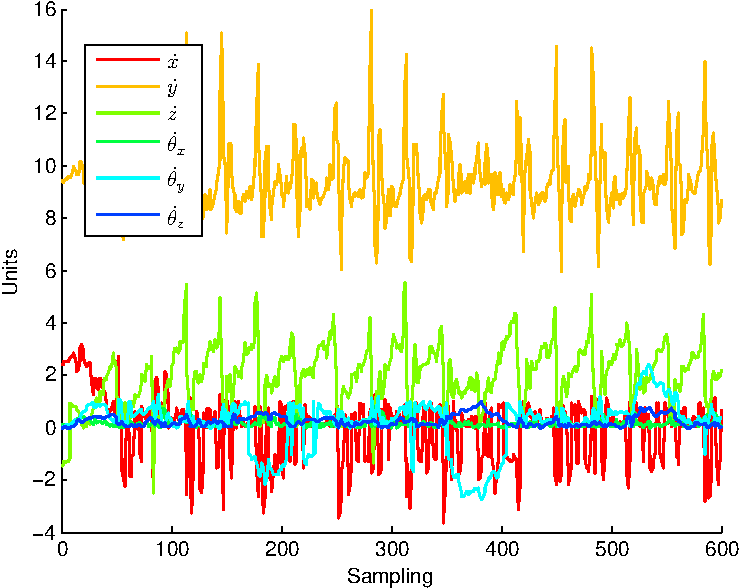
\includegraphics[width=0.32\textwidth]{plots/human_walk-crop.pdf}} 
\subfloat[Human stand to seat.]{\label{fig:hb}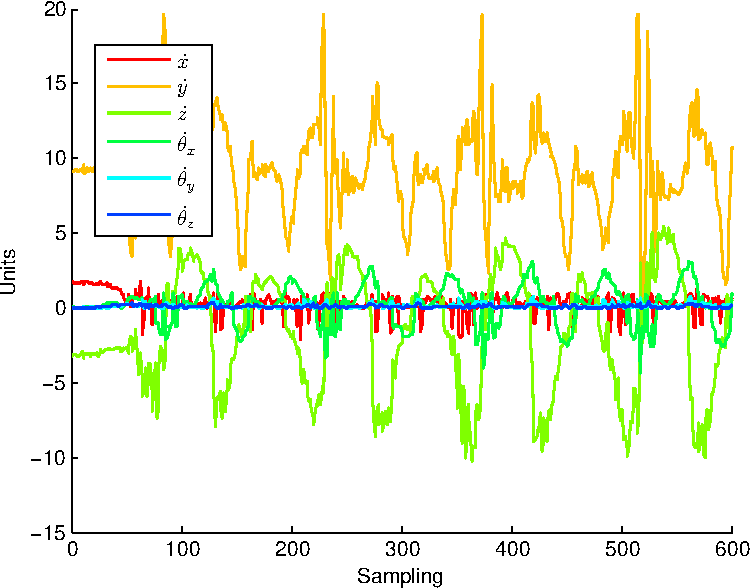
\includegraphics[width=0.32\textwidth]{plots/human_stand-crop.pdf}}
\subfloat[Human stand to fall.]{\label{fig:hc}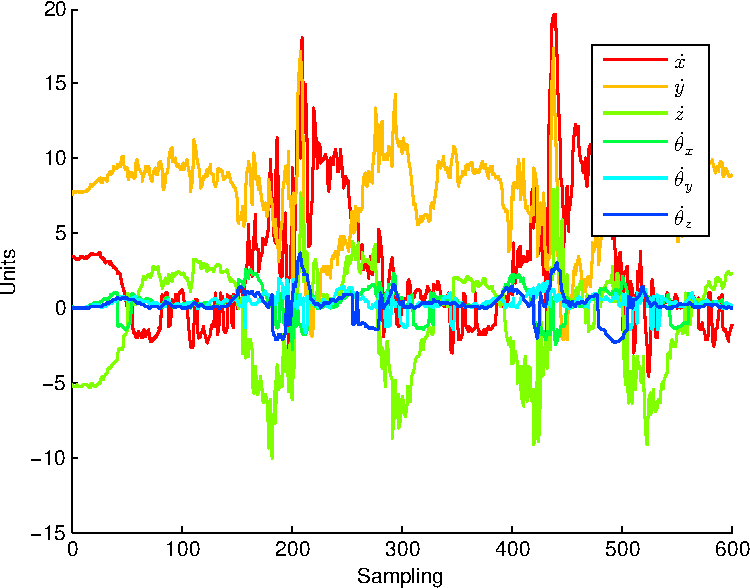
\includegraphics[width=0.32\textwidth]{plots/human_falling-crop.pdf}}
\\
\subfloat[Robot walk forward.]{\label{fig:ha}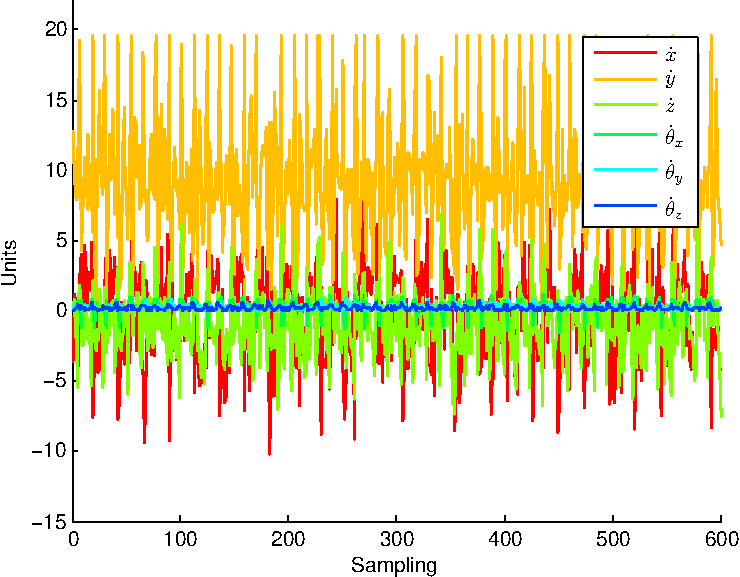
\includegraphics[width=0.32\textwidth]
{plots/robot_walk_forward-crop.pdf}}
\subfloat[Robot walk backward.]{\label{fig:hb}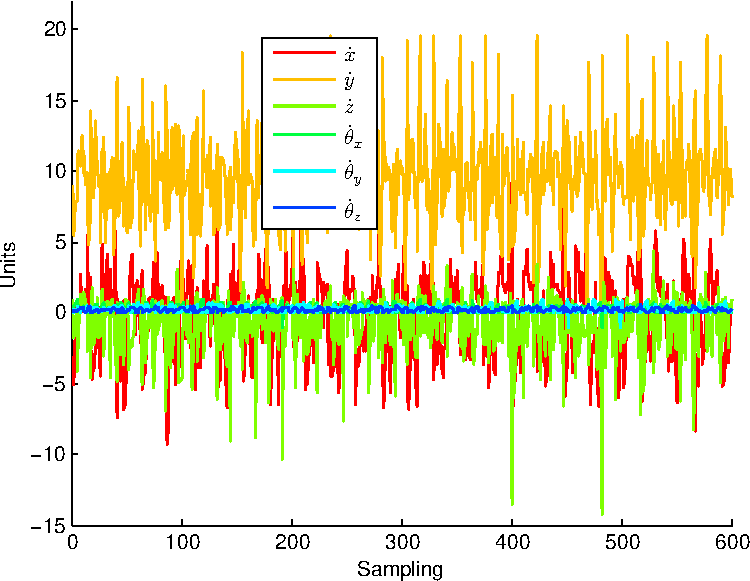
\includegraphics[width=0.32\textwidth]
{plots/robot_walk_backward-crop.pdf}}
\subfloat[Robot rotate clockwise.]{\label{fig:hc}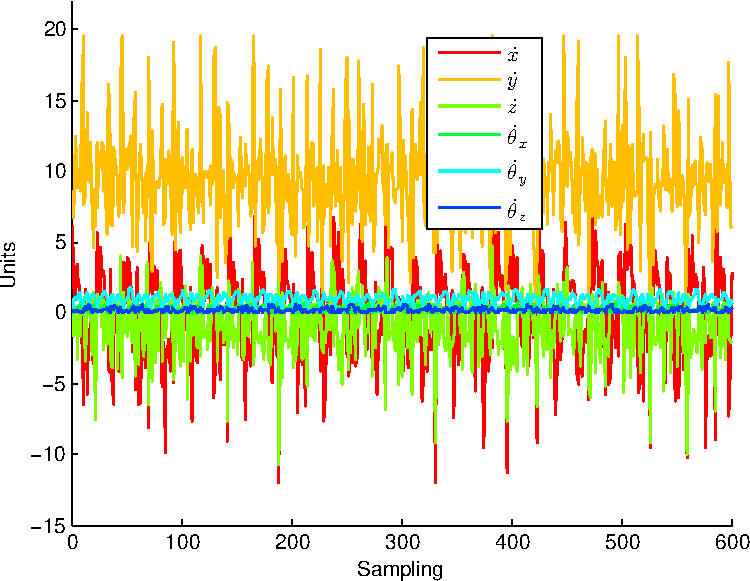
\includegraphics[width=0.32\textwidth]
{plots/robot_rotate_cw-crop.pdf}}
\\
\subfloat[Robot fallen forward.]{\label{fig:ha}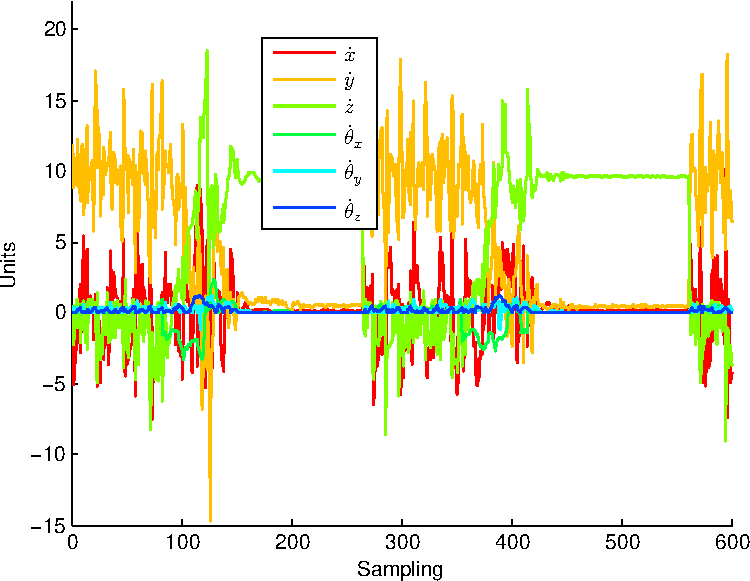
\includegraphics[width=0.32\textwidth]
{plots/robot_fallen_forward-crop.pdf}} 
\subfloat[Robot fallen backward.]{\label{fig:hb}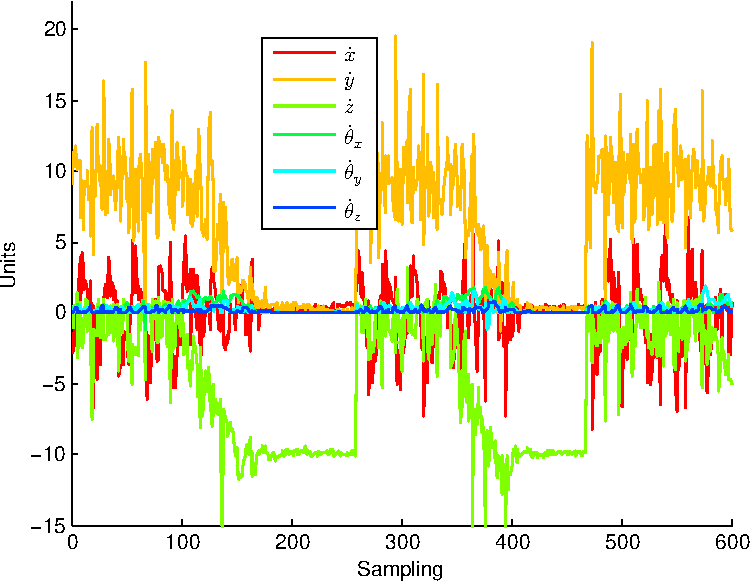
\includegraphics[width=0.32\textwidth]
{plots/robot_fallen_backward-crop.pdf}}
\subfloat[Robot fallen right.]{\label{fig:hc}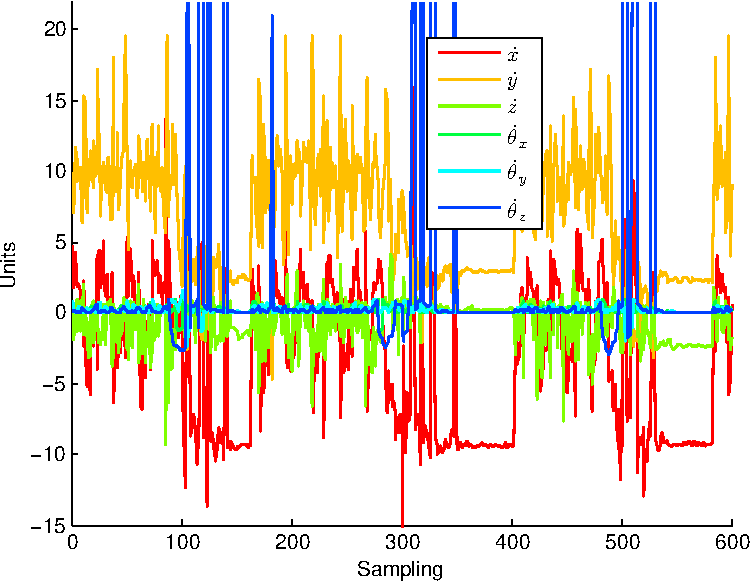
\includegraphics[width=0.32\textwidth]
{plots/robot_fallen_right-crop.pdf}}

\caption{Figures (a)-(c) shows 3-axis accelerometer and 3-axis gyroscope graph for human motions. Figures (d)-(f) shows 3-axis accelerometer and 3-axis gyroscope graph for robot's walk motion. Figures (g)-(i) shows 3-axis accelerometer and 3-axis gyroscope graph for robot's fallen motion}
 \label{fig:anotation-human-robot} 
\end{figure*}


We have conducted experiments on detecting motions (activities) on 
%able-bodied 
humans and a humanoid robot (NAO robot). We have used InvenSense MPU-9150 
motion tracking sensor on the sensor hub. The module {\em MPU9150Module} connects to this device
and provides the representation {\em MPU9150Representation}. The representation contains
3-axis accelerometer readings, 3-axis gyroscope readings, 3-axis magnetometer readings, the quaternion
rotation axis of the device, and Euler angles roll, pitch, and yaw.  In order to calculate Euler
angles, we have used the Direction Cosine Matrix (DCM) algorithm.  Depending on the
experiment, the practitioner can change the sampling rate of the sensor.  The maximum sampling rate
of the sensor is 1,000$Hz$. This section shows our results, validations, and conclusions.


\subsection{Activity Annotation}

The annotation for different human and robot motion events are shown in Fig.{~\ref{fig:anotation-human-robot}}. 
Accelerometer and gyroscope's X, Y and Z axis are shown for different motions. We can observe that an 
actual event takes between 180--250 ms. Figure{~\ref{fig:anotation-human-robot}}(a)-(c) shows the activity 
annotations for human motions (walking forward, sitting down, falling down). Fig.{~\ref{fig:anotation-human-robot}}
(d)-(i) shows activity annotations for the NAO robot. We have structured the text in a way that we discuss 
data processing, machine learning and results for both the human and robotic experiments.

\subsection{Experiments with a Human}
\subsubsection{Data processing:} 
We have collected data for different human activities. We have put the sensors on the back of the
human body (cf. figure \ref{fig:fb}) and collected data from those sensors in fixed interval. 
We have sampled data at 50$Hz$ for our experiments. We sampled from several different human configurations:
\begin{inparaenum}[(1)] \item walking forward; \item from standing to sitting down and back to standing;
and \item from standing to falling and back to standing\end{inparaenum}. Since we have used a 9-axis MEMS device 
each sample contains accelerometer readings in three-axis in $ms^{-2}$, gyroscope readings in 
three-axis in $rads^{-2}$, and magnetometer readings in three-axis in {\em Tesla}. 

An activity consists of multiple sensor readings since it is not sufficient to detect activities based 
on a single reading. We have used a 200$ms$ time-frame-based prediction protocol, which entails that we
predict an event with all the sensor readings within that time frame. 

If our detection procedure detects an event for more than 90\% of the defined time frame, we denote that 
event as a \textit{true} event. We use two classifiers for this detection: \begin{inparaenum}[1)] 
\item logistic regression; and \item support vector machines (SVM)\cite{Bishop:2006:PRM:1162264}. 
\end{inparaenum} 
We have used standard parameter sweeping techniques to find the classifier parameters that provide 
the best trade-off between the bias and the variance, while precision, recall, and F$_1$-scores have 
been used to obtain the best value. As a preprocessing step, the features, except the bias, have 
been subjected to feature standardization. We have independently set each dimension of the sample 
to have zero-mean and unit-variance. We achieved this by first computing the mean of each dimension 
across the dataset and subtracting this from each dimension. Then each dimension is divided by its 
standard deviation.

\subsubsection{Machine Learning\\}
\emph{Classification using Logistic Regression:}
In the first part of the data analysis we have put all our collected samples together and labeled it
with specific number to denote the position. We have used a multivariate logistic regression model to
classify our samples. We have used 80\% of the samples for training, while the rest has been used
for the cross-validation process. Table \ref{tab:human-logistic-class} shows the final results, where, TP, TN, 
FP, and FN stand for true positive, true negative, false positive, and false negative respectively. 

\begin{table}[!ht]
\caption{Logistic regression classification for human activities.}
	\label{tab:human-logistic-class}
	\centering
		\begin{tabular} {|l |c |c |c|c|}
			\hline
			{\bf Activity} & {\bf  TP}  &	{\bf TN}  &	{\bf FP} &	{\bf FN} \\ 
			\hline
			Walking	& 88\%	& 84\%	& 16\%	& 12\% \\ \hline
			Stand to seat	& 92\%	& 82\%	& 18\% & 	8\%	 \\ \hline 
			Stand to fall	& 92\%	& 88\%	& 12\%	& 8\%	 \\ \hline
		\end{tabular}
\end{table}

\noindent\emph{Classification and Validation using Support Vector Machine:}
In the second part of the data analysis we have used a SVM model
to classify our samples. To train the model, we used the same protocol as before; 80\% of
samples were used to train the classifier and the rest of the  samples were used for 
cross-validation. Table \ref{tab:human-svm-class} shows the final results.

\begin{table}[!ht]
\caption{SVM classification for human activities.}
	\label{tab:human-svm-class}
	\centering
		\begin{tabular} {|l |c |c |c|c|}
			\hline
			{\bf Activity} & {\bf  TP}  &	{\bf TN}  &	{\bf FP} &	{\bf FN} \\ 
			\hline
			Walking	& 92\%	& 86\%	& 14\%	& 8\% \\ \hline
			Stand to seat	& 94\%	& 84\%	& 16\% & 	6\%	 \\ \hline 
			Stand to fall	& 98\%	& 88\%	& 12\%	& 2\%	 \\ \hline
		\end{tabular}
\end{table}

\subsubsection{Results:}
Our experiments reveal that the SVM classifier performs better than the logistic regression classifier. 
However, due to memory and computational restrictions on the humanoid robot, we have found that the logistic 
regression classifier is a better choice. We assume that the same observation can be made on most embedded 
devices. Our feature vector consists of the mean normalized sensor reading and a bias term. We plan to 
combine and prune features to improve the classification accuracy for future work.  


\subsection{Humanoid Robot NAO}
\subsubsection{Data processing:} 
We have used the device configuration as described in section \ref{sec:Intro}
and it was attached to the robot as shown in Figure \ref{fig:fc}. In the first experiment, we have 
designed a thresholding base activity predictor. We have calculated the roll, pitch, and yaw angles 
for this study (the roll is around the x-axis, the pitch is around the y-axis, and the yaw is around 
the z-axis). We also have configured the InvenSense MPU-9150 motion sensor on the sensor hub to 
sample data at 50$Hz$. We have chosen this value to compensate delays in communications and to cope 
with the constraints provided by the robot. We have focused on detecting the following motions: \textit{marching}, \textit{walking forward/backward}, \textit{turning clockwise/counter-clockwise},
as well as \textit{falling back}, \textit{falling front}, and \textit{falling sideways}.

\begin{figure*}[!ht]
  \centering
  \subfloat[Marching in place.]{\label{fig:tsnedataset_1}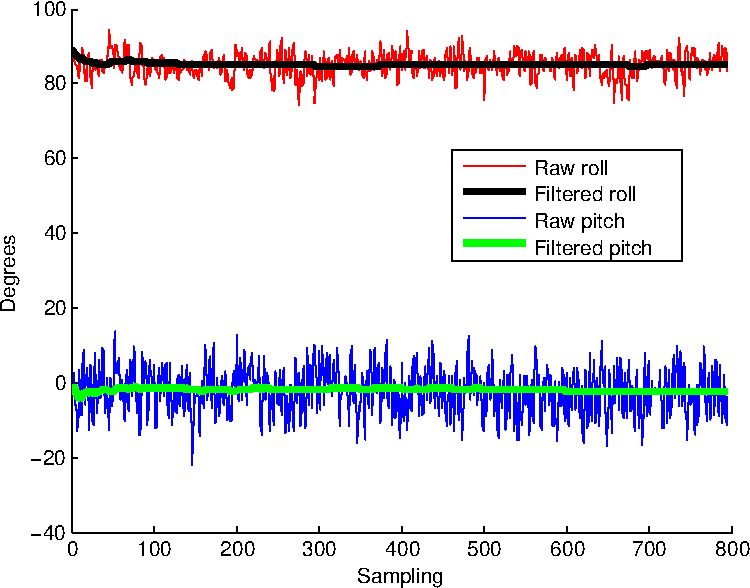
\includegraphics[width=0.25\textwidth]
       {plot1-crop}} 
  \subfloat[Walking backward.]{\label{fig:tsnedataset_9}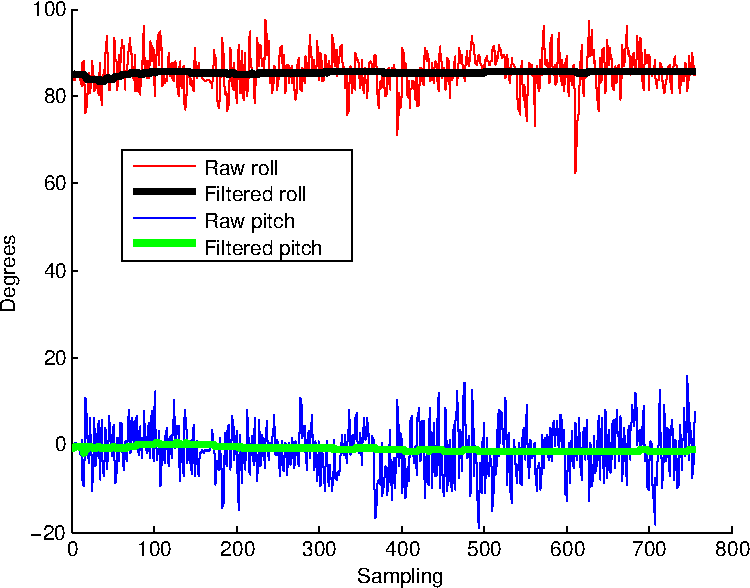
\includegraphics[width=0.25\textwidth]
       {plot5-crop}}
  \subfloat[Rotating clockwise.]{\label{fig:tsnedataset_7}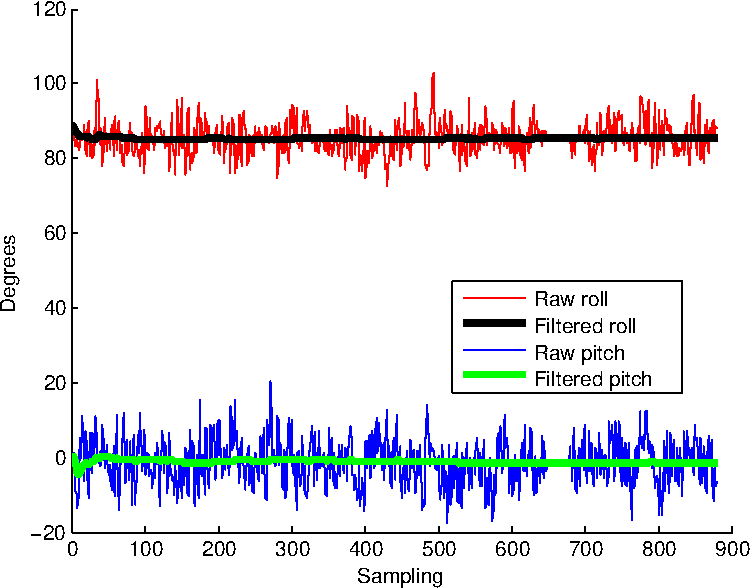
\includegraphics[width=0.25\textwidth]
       {plot2-crop}}
  \subfloat[Left side-way walk.]{\label{fig:tsnedataset_10}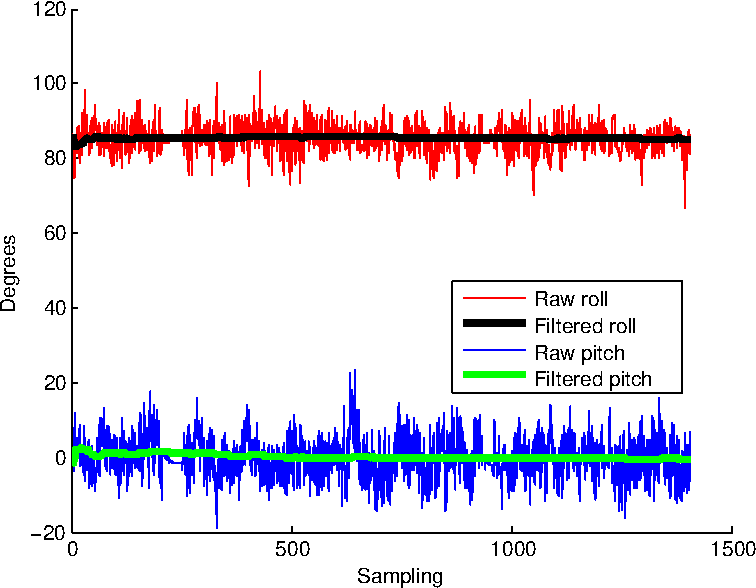
\includegraphics[width=0.25\textwidth]
       {plot6-crop}}
       \\
  \subfloat[Falling forward.]{\label{fig:tsnedataset_11}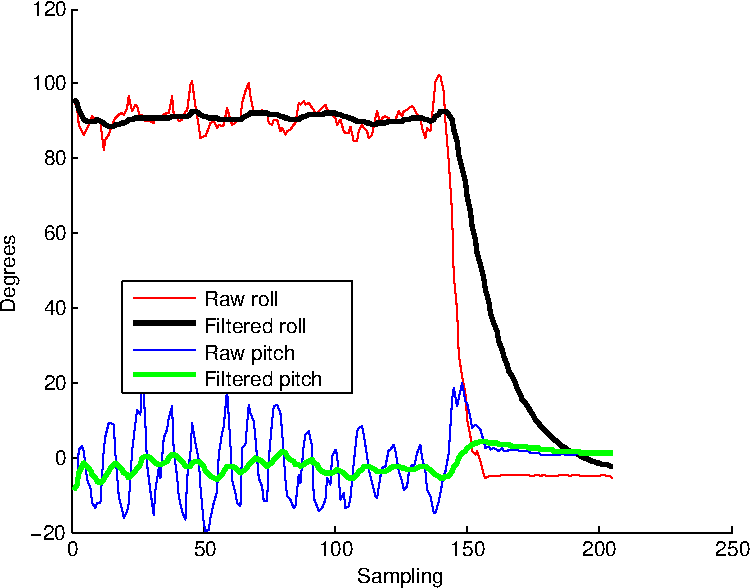
\includegraphics[width=0.25\textwidth]
       {plot1_fallen-crop}}
  \subfloat[Falling backward.]{\label{fig:tsnedataset_12}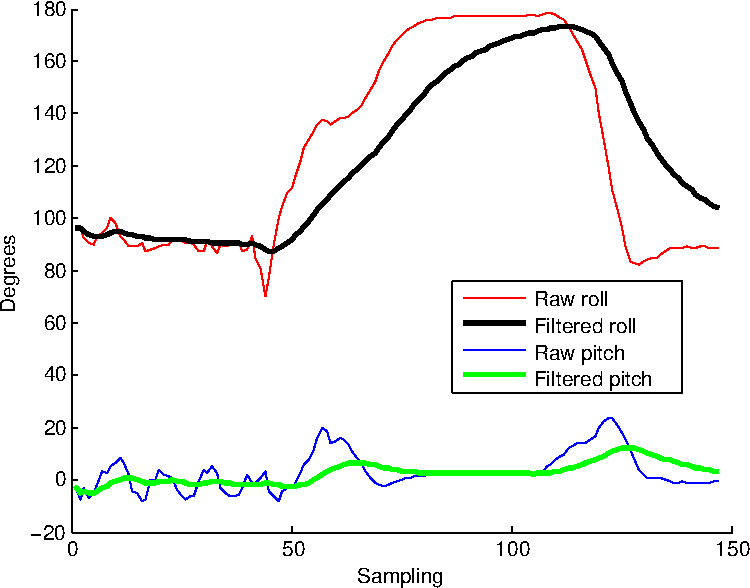
\includegraphics[width=0.25\textwidth]
       {plot2_fallen-crop}}
  \subfloat[Falling to left side.]{\label{fig:tsnedataset_13}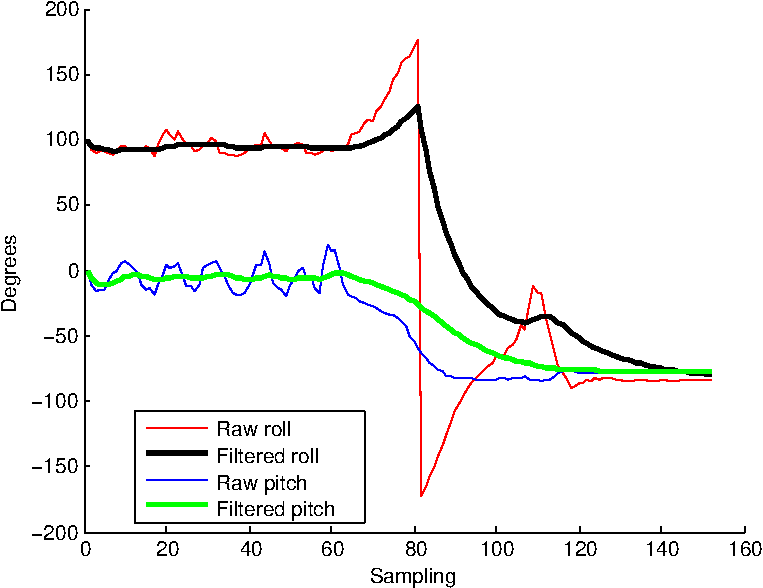
\includegraphics[width=0.25\textwidth]
       {plot3_fallen-crop}}
  \subfloat[Falling to right
side.]{\label{fig:tsnedataset_14}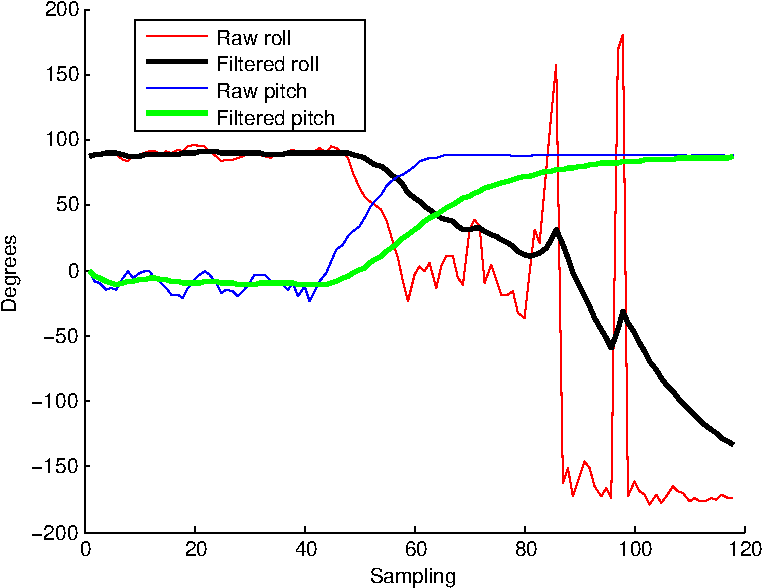
\includegraphics[width=0.25\textwidth]
       {plot4_fallen-crop}}      
  \caption{Figures (a)-(d) show the roll and pitch angles (raw and filtered) for normal 
behavior. Figures (e)-(h) show the raw and filtered roll and pitch angles for fallen 
states of NAO humanoid robot.}
  \label{fig:normalFallenBehavior}

\end{figure*}

Our NAO robots have an omni-directional walking engine to conduct walking motions.  
These motions are regulated by linear velocities $\dot{x}_v$ and $\dot{y}_v$, and an 
angular velocity $\dot{\theta}_v$ as input parameters. Depending on these
values we can let the robot walk (forward, backward, and side-ways) and rotate (clockwise and
counter-clockwise) with different speeds. In this study we have considered \begin{inparaenum}[(1)]
\item marching ($\dot{x}_v = 0 , \dot{y}_v = 0, \dot{\theta}_v = 0$); \item walking  
forward/backward ($\dot{x}_v = \pm200
, \dot{y}_v = 0, \dot{\theta}_v = 0$);  \item walking side-ways ($\dot{x}_v = 0, \dot{y}_v = 
\pm200, \dot{\theta}_v = 0$); and  \item rotating clockwise/counter-clockwise
($\dot{x}_v = 0 , \dot{y}_v = 0, \dot{\theta}_v = \pm 0.5$) \end{inparaenum} as {\em normal states}, 
while all the other activities are classified as {\em fallen states}. We have used the  
following protocol to collect samples. \textit{Firstly}, we set the velocity parameters and use the wireless 
radio to transmit the samples to the sample-collection device. \textit{Secondly}, we activate the robot to 
the given configuration. \textit{Finally}, we have tagged the start point of the sample stream and waited 
approximately a minute to tag the end of the sample stream. This is an episode of the normal state. 
We have collected multiple episodes to create our learning ensemble. To collect samples for fallen 
states, we have configured the robot to march. Then, we safely pushed the robot to 
different directions to inducing the fallen state. Similarly, we tagged the sample streams to 
generate episodes.    

\begin{table}[!ht]
\caption{Logistic regression classification for robot activities.}
	\label{tab:robot-logistic-class}
	\centering
		\begin{tabular} {| l | c | c | c| c|}
		\hline
			{\bf Activity} & {\bf  TP}  &	{\bf TN}  &	{\bf FP} &	{\bf FN} \\ 
\hline
			Walking forward	& 86\%	& 84\%	& 16\%	& 14\% \\ \hline
			Walking backward	& 86\%	& 84\%	& 16\%	& 14\% \\ \hline
			Walking left 	& 88\%	& 86\%	& 14\%	& 12\% \\ \hline
			Walking right 	& 86\%	& 84\%	& 16\%	& 14\% \\ \hline
			Falling forward	& 94\%	& 90\%	& 10\%	& 6\%	 \\ \hline
			Falling Backward	& 94\%	& 88\%	& 12\%	& 6\%	 \\ \hline
			Falling left	& 92\%	& 92\%	& 8\%	& 8\%	 \\ \hline
			Falling Right	& 92\%	& 92\%	& 8\%	& 8\%	 \\ \hline
			Marching	& 88\%	& 84\%	& 16\%	& 12\%	 \\ \hline
			Rotate counter-clockwise	& 94\%	& 90\%	& 10\%	& 6\%	 \\ \hline
			Rotate clockwise	& 94\%	& 90\%	& 10\%	& 6\%	 \\ \hline
		\end{tabular}
\end{table}

We have used the roll and pitch values to detect relevant activities. In order to achieve 
an effective threshold-based decision making we have filtered the roll, pitch, and
yaw values using a Kalman filter \cite{Welch:1995:IKF:897831}. Figures 
\ref{fig:normalFallenBehavior} ((a)--(d)) show
the raw and the filtered values of the raw and the pitch values for marching, walk backward,
rotating clockwise, and left side-way walk. The other activities show similar plots (we have 
refrained from plotting them due to space constraints). The thresholding method
suggests that, if the filtered roll values are within the range $[90\pm15]$ (degrees) and the
filtered pitch values are within the rage $[0\pm15]$ (degrees), then with 100\% accuracy, NAO 
humanoid robot will is in a normal state. Otherwise, we can safely assume that the robot is in 
a fallen state.   

We have defined four fallen states for the robot: \begin{inparaenum}[(1)] \item falling
forward; \item falling backward; \item falling to left side; and \item falling to right
side\end{inparaenum}. Figures \ref{fig:normalFallenBehavior} ((e)--(h)) show the roll and pitch 
angles (raw and filtered) for typical fallen robot. If the filtered roll value is less that 60 
degrees, we can safely assume that the robot is falling forward. If the filtered roll values is 
more than 100 degrees we can assume that the robot is falling backward. To detect the events 
falling to the left and right, we have used the filtered pitch values. If the filtered pitch value 
is less than -50 degrees, we can assume that the robot is falling to the left side, while if the 
filtered pitch values is more than 50 degrees, we can assume that the robot is falling to the right 
side. With these thresholds for a separate test cases, the thresholding method has detected fallen 
state with 100\% accuracy. 

\subsubsection{Machine Learning:}
Even though thresholding method successfully distinguished between normal and fallen states, it was 
unable to detect states within normal activities, i.e., walking forward to waling backward so 
forth. Therefore, similar to the previous experiments, we have used logistic regression and SVM 
classifiers to identify different activities. We have followed the same protocols as mentioned in 
the previous section to generate features, learning, and prediction. Table 
\ref{tab:robot-logistic-class} shows the results for the logistic regression classifier, while, 
Table \ref{tab:robot-svm-class} shows the results for the SVM classification. We conclude that the 
classification methods are able to predict activities within normal states as well as fallen 
states. Similar to previous section, the SVM classifier performs better that the logistic 
regression classifier, though, during operation, we prefer the logistic regression classifier.   


\begin{table}[!ht]
\caption{SVM classification for robot activities.}
	\label{tab:robot-svm-class}
	\centering
		\begin{tabular} {| l | c | c | c | c | }
		\hline
			{\bf Activity} & {\bf  TP}  &	{\bf TN}  &	{\bf FP} &	{\bf FN} \\ 
\hline
			Walking forward	& 90\%	& 88\%	& 12\%	& 10\% \\ \hline
			Walking backward	& 90\%	& 88\%	& 12\%	& 10\% \\ \hline
			Walking left	& 92\%	& 86\%	& 14\%	& 8\% \\ \hline
			Walking right	& 92\%	& 86\%	& 14\%	& 8\% \\ \hline
			Falling forward	& 96\%	& 90\%	& 10\%	& 4\%	 \\ \hline
			Falling backward	& 96\%	& 88\%	& 12\%	& 4\%	 \\ \hline
			Falling left	& 94\%	& 92\%	& 8\%	& 6\%	 \\ \hline
			Falling right	& 94\%	& 92\%	& 8\%	& 6\%	 \\ \hline
			Marching	& 90\%	& 88\%	& 12\%	& 10\%	 \\ \hline
			Rotate counter-clockwise	& 96\%	& 90\%	& 10\%	& 4\%	 \\ \hline
			Rotate clockwise	& 96\%	& 90\%	& 10\%	& 4\%	 \\ \hline
		\end{tabular}
\end{table}

\subsubsection{Results:} 
The range of motion of NAO humanoid robot is comparatively constrained compared to a able-bodied 
human. Therefore, we only conduct primary activities as described in this section. We have not 
conducted experiments on activities such as stand to seat. When determining the results, we 
have sampled the motion device data at the rate 50$Hz$. During operation, if the 
thresholding method is used, we can use the same thresholds with higher sampling rate. The second 
method requires learning for different sampling rates.



\section{Conclusion and Future Work}

We have proposed framework to write heterogeneous applications on TIs microcontrollers. We have used 
our framework to detect and predict activities on able-bodied humans and NAO humanoid robots. We 
have shown that our methods are capable of detecting events with high accuracy. We have used 
machine learning methods and thresholding methods to detect different events and provided 
justifications for the success of the applications. Comparing the encouraging experimental results 
achieved, our future work will be to use multiple devices to create a sensor network to detect 
complex and minute activities with higher sampling rates.  

\bibliographystyle{aaai}
\bibliography{references}


\end{document}
